\section{Model Component} \label{sc:model_component}
Based on the analysis of the problem domain (see \autoref{ch:problemdomain}), through the class diagram, event table, and state charts, the model component of the system has been constructed.
\par
Additional classes, attributes, and structures have been defined to support the mentioned events and the desired functionality of the system. The result is an updated class diagram that contains attributes, operations, and additional classes and structures.

\subsection{Additional classes}
To sufficiently solve the problems in the problem domain, additional classes were needed and have been described.
\par

\subsubsection{\textit{Tag} and \textit{Asset-tag relation}}
During the interviews, Aalborg Zoo mentioned a potential organisational structure to ease the use of the system (see \autoref{ch:problemdomain}). This structure is based on tags, which can be attached to assets and used to filter and add details to these.
The structure adds the \textit{Tag} and \textit{Asset-tag relation} classes to the system. 
\par
A tag will either belong to a department or be available to all departments \autoref{fig:TagAndAsset-TagRelationWithAttributes}.
\par
The \textit{Asset-tag relation} class has been added to represent a connection between an asset and a tag, as an asset can have multiple tags related to it and a tag can be related to multiple assets.
\par

\begin{figure}[H]
    \centering
    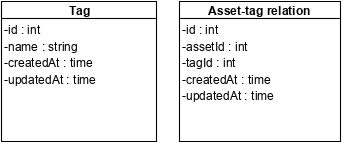
\includegraphics[width=0.55\textwidth]{figures/Classes/TagAndAsset-tagRelationWithAttributes.png}
    \caption{Overview of the \textit{Tag} a \textit{Asset-tag relation} classes with attributes}
    \label{fig:TagAndAsset-TagRelationWithAttributes}
\end{figure}


\subsubsection{\textit{Field}}
To help declutter the application and fulfill the requirement to only fill in relevant information intuitively, the \textit{Field} class is introduced \autoref{fig:FieldWithAttributes}). Both assets and tags can contain the \textit{Field} class. If a field is contained by a tag and that tag is attached to an asset, the field is transferred to the asset as well. Fields only exist in an asset or a tag and never on its own.
\par
The field has certain attributes unique to the class:
\begin{itemize}
    \item \textbf{Type} that defines what kind of input it takes. This can be a text box, a text area, a number, a date, or a checkbox.
    \item \textbf{Content} which will hold the value set by the user.
    \item \textbf{Required} which defines whether or not the field must be filled in before saving the asset
\end{itemize}

\begin{figure}[H]
    \centering
    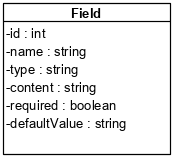
\includegraphics[width=0.28\textwidth]{figures/Classes/FieldAttributes.png}
    \caption{Overview of the \textit{Field} class with attributes}
    \label{fig:FieldWithAttributes}
\end{figure}


\subsubsection{\textit{Comment}}
To allow the users to comment on assets in the system, a \textit{Comment} class has been introduced. A comment is attached to an asset and contains the ID and name of the asset, the username of the user, whom the comment was created by, a comment text, and timestamps for its creation and last update (see \autoref{fig:CommentWithAttributes}).

\begin{figure}[H]
    \centering
    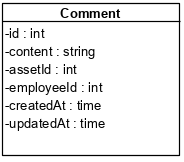
\includegraphics[width=0.28\textwidth]{figures/Classes/CommentAttributes.png}
    \caption{Overview of the \textit{Comment} class with attributes}
    \label{fig:CommentWithAttributes}
\end{figure}


\subsubsection{\textit{FieldContainer}}
To ensure that both the asset and tag classes have a list of fields and has the correct properties and functionality, an abstract class has been implemented called \textit{FieldContainer}. Both the asset and tag classes are specializations of this abstract class (see \autoref{fig:FieldContainer}).

\begin{figure}[H]
    \centering
    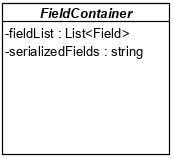
\includegraphics[width=0.28\textwidth]{figures/Classes/FieldContainer.png}
    \caption{Overview of the \textit{FieldContainer} class with attributes}
    \label{fig:FieldContainer}
\end{figure}


\subsubsection{\textit{User}}
To model the users in the system, the class \textit{User} was added. This class contains information about the user, such as username, as well as the users domain (see \autoref{fig:User}).

\begin{figure}[H]
    \centering
    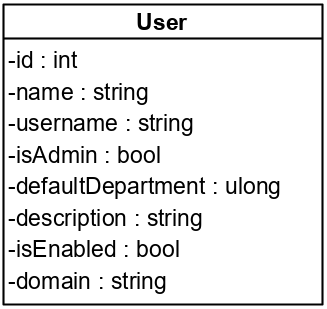
\includegraphics[width=0.28\textwidth]{figures/Classes/User.png}
    \caption{Overview of the \textit{User} class with attributes}
    \label{fig:User}
\end{figure}

Based on these additional classes, the \textit{Employee}, \textit{Admin}, and \textit{Loan} classes needed a revision.
\par
The \textit{Employee} and \textit{Admin} classes have been used to store information about the system's users. This is covered by the \textit{User} class, which also stores information about whether or not that user is an admin.
\par
Aside from this, the \textit{Loan} class has been used to keep track of who is in possession of which assets. This functionality can be covered by the \textit{Tag} class, as it can act as the relation between an asset and a user, by containing the username of the user as its label. This means that an asset can have tags attached, containing the usernames of the employees currently in possession of it.
\par
The other functionality of the \textit{Admin} class has been to identify whether the logged in user has access to administrator functionality or not. This function is handled by the \textit{Session} class, which will be explained in the function component (see \autoref{sc:function_component}).
\par
Based on these changes, the \textit{Admin}, \textit{Employee}, and \textit{Loan} classes from the problem domain have become obsolete and will therefore not be taken into consideration when designing the system.

\subsection{Attributes of problem domain classes}
To ensure that every event and functionality is supported, the following attributes have been added to the classes from the class diagram in the problem domain (see \autoref{fig:FirstPDClassDiagram}).
\par
Throughout this subsection only attributes needing further explanation will be mentioned. Full attribute lists can be found in the related figures of the classes.

\subsubsection{Asset attributes}
An asset has a timestamp of its deletion. This is used for soft deletion, which works as an extra step to avoid unwanted deletes. Soft deletion works by marking an asset with a deletion date, instead of removing the element from the database entirely. This allows the asset to be recovered, if it is accidentally deleted (see \autoref{fig:AssetWithAttributes}).

\begin{figure}[H]
    \centering
    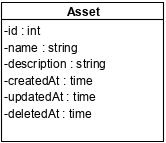
\includegraphics[width=0.28\textwidth]{figures/Classes/AssetAttributes.png}
    \caption{Overview of the \textit{Asset} class with attributes}
    \label{fig:AssetWithAttributes}
\end{figure}

\subsubsection{Department attributes}
The \textit{Department} class does not contain any nontrivial attributes, and can be see in \autoref{fig:DepartmentWithAttributes}.
\begin{figure}[H]
    \centering
    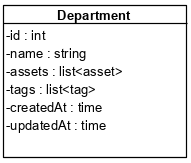
\includegraphics[width=0.28\textwidth]{figures/Classes/DepartmentAttributes.png}
    \caption{Overview of the \textit{Department} class with attributes}
    \label{fig:DepartmentWithAttributes}
\end{figure}


\subsection{Structures}
The events and relations not completely supported by the classes and attributes described previously in this section will be achieved with the following structures of classes.

\subsubsection{Assets and tags can contain fields}
Both the \textit{Asset} and the \textit{Tag} classes aggregates the \textit{Field} class. An asset or a tag can contain multiple fields, but a field belongs to only one asset or one tag. To ensure that both classes have a list of fields and implement the correct properties, they both specialize the abstract class \textit{FieldContainer} (see \autoref{fig:AssetTagFieldStructure}).

\begin{figure}[H]
    \centering
    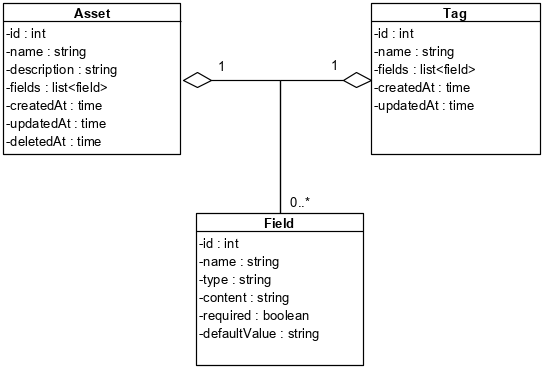
\includegraphics[width=0.65\textwidth]{figures/Structures/AssetTagFieldStructure.png}
    \caption{Overview of the structure between the \textit{Asset}, \textit{Tag}, \textit{FieldContainer}, and \textit{Field} classes}
    \label{fig:AssetTagFieldStructure}
\end{figure}

\newpage

\subsubsection{An asset contains comments}
An asset can be commented on, which attaches the comment to the asset. An asset can have multiple comments, but a comment can only be attached to one asset (see \autoref{fig:AssetCommentStructure}). 
\par
The comments could be implemented as a list on the asset. However, because the comments will be shown in parts of the system without the assets, the aggregation makes it possible to only fetch the comments and sort through these, without having to fetch all the assets as well.

\begin{figure}[H]
    \centering
    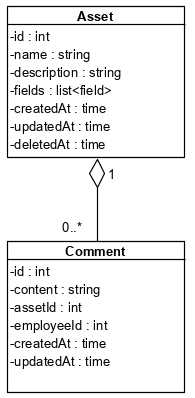
\includegraphics[width=0.25\textwidth]{figures/Structures/AssetCommentStructure.png}
    \caption{Overview of the structure connecting the \textit{Asset} and \textit{Comment} classes}
    \label{fig:AssetCommentStructure}
\end{figure}

% \subsubsection{Tag relation between asset and tag}
% Between the \textit{Tag} and \textit{Asset} classes is a many-to-many relation, which has been replaced by the class \textit{Tagged}. An asset can have multiple tag relations attached to it, as tags can be added to the asset dynamically. A tag does also have multiple tag relations connected to is, as a tag can be attached to multiple assets.

% \begin{figure}[H]
%     \centering
%     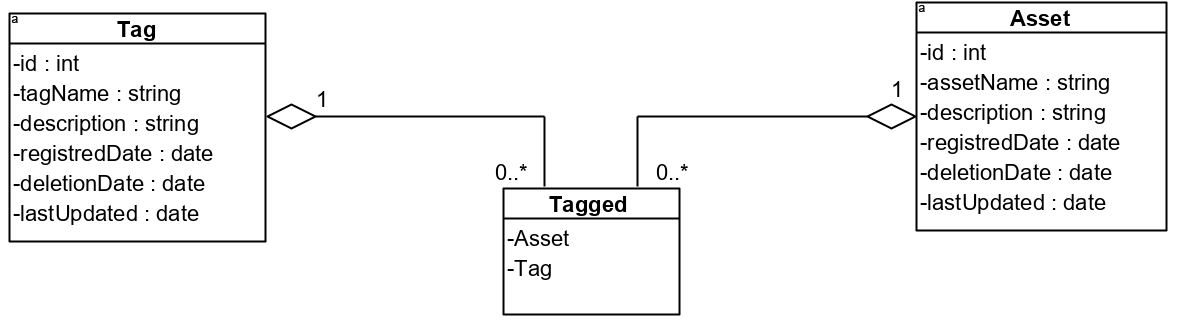
\includegraphics[width=0.8\textwidth]{figures/Structures/TagAssetRelation.PNG}
%     \caption{Overview of the asset class}
%     \label{fig:TagAssetRelation}
% \end{figure}

\subsubsection{A department contains assets and tags}
Assets and tags are added to a department, as they are created. An asset belongs to exactly one department, while a tag belongs to one or all departments. A department contains multiple assets and tags (see \autoref{fig:DepartmentAssetTagStructure}). The tag is depicted to belong to non or 1 department. This should be read as a tag either belongs to one department or belongs to none. When a tag belongs to non, it becomes available to all.

\begin{figure}[H]
    \centering
    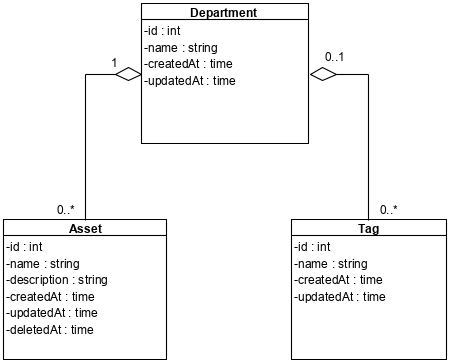
\includegraphics[width=0.7\textwidth]{figures/Structures/DepartmentAssetTagStructure.png}
    \caption{Overview of the structure between the \textit{Department}, \textit{Asset}, and \textit{Tag} classes}
    \label{fig:DepartmentAssetTagStructure}
\end{figure}

\subsubsection{Parent tags}
To make the tagging more manageable, the ability to group tags has been introduced, mimicking a hierarchical folder structure. This is accomplished through parent tags. By doing this, a parent tag can contain multiple tags, which are seen as its children. 
\par
A tag can only either belong to one parent tag or be a parent tag itself. This means that there is no single tag that can act as both parent and child tag. As a product of this, the structure becomes a two level hierarchy (see \autoref{fig:TagHierarchy}). 
\par
The figure (see \autoref{fig:TagHierarchy}) is only an illustration of the relation between two tags. In the system the two classes exist as the \textit{Tag} class, with the relation represented by an attribute linking the child tag to the parent.

\begin{figure}[H]
    \centering
    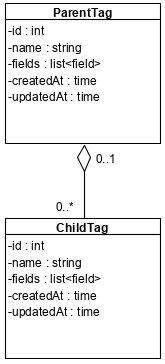
\includegraphics[width=0.28\textwidth]{figures/Structures/TagHierarchy.png}
    \caption{Overview of the structure of the \textit{ParentTag} and \textit{ChildTag} classes}
    \label{fig:TagHierarchy}
\end{figure}

\newpage

\subsection{Updated class-diagram}
The additions mentioned above have added up to the following class-diagram, which represents the model component, and can be seen in \autoref{fig:ModelComponentClassDiagram}.

% Tags og andre ting skal introduceres inden dette afsnit
\begin{figure}[H]
    \centering
    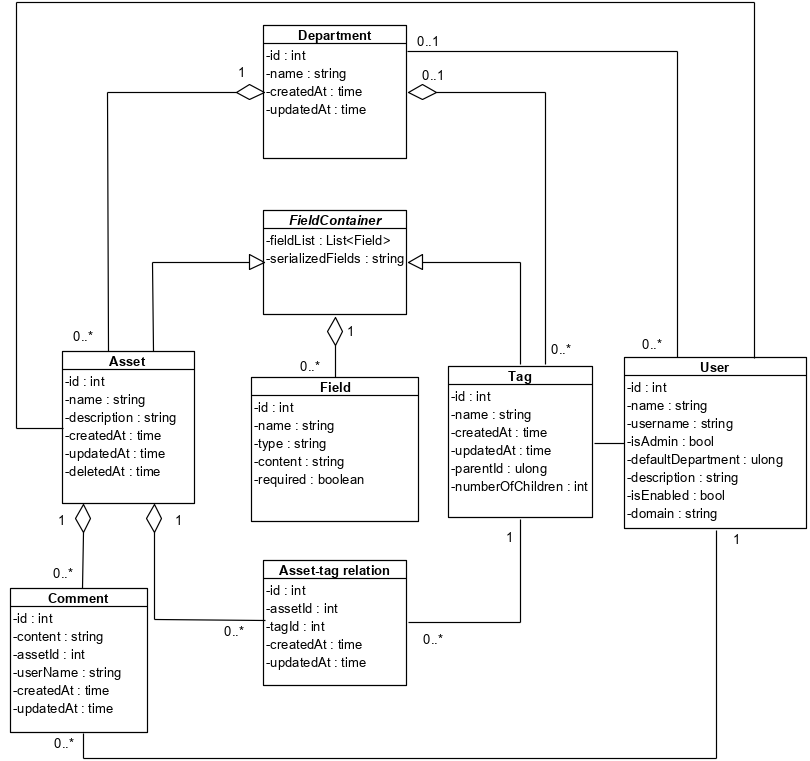
\includegraphics[width=0.9\textwidth]{figures/ClassDiagrams/ModelComponentClassDiagram.png}
    \caption{Class diagram for the model component}
    \label{fig:ModelComponentClassDiagram}
\end{figure}
